%%%%%%%%%%%%%%%%%%%%%%%%%%%%%%%%%%%%%
%                                   %
% Compile with XeLaTeX and biber    %
%                                   %
% Questions or comments:            %
%                                   %
% joshua dot mcneill at uga dot edu %
%                                   %
%%%%%%%%%%%%%%%%%%%%%%%%%%%%%%%%%%%%%

\documentclass{beamer}
  % Read in standard preamble (cosmetic stuff)
  %%%%%%%%%%%%%%%%%%%%%%%%%%%%%%%%%%%%%%%%%%%%%%%%%%%%%%%%%%%%%%%%
% This is a standard preamble used in for all slide documents. %
% It basically contains cosmetic settings.                     %
%                                                              %
% Joshua McNeill                                               %
% joshua dot mcneill at uga dot edu                            %
%%%%%%%%%%%%%%%%%%%%%%%%%%%%%%%%%%%%%%%%%%%%%%%%%%%%%%%%%%%%%%%%

% Beamer settings
% \usetheme{Berkeley}
\usetheme{CambridgeUS}
% \usecolortheme{dove}
% \usecolortheme{rose}
\usecolortheme{seagull}
\usefonttheme{professionalfonts}
\usefonttheme{serif}
\setbeamertemplate{bibliography item}{}

% Packages and settings
\usepackage{fontspec}
  \setmainfont{Charis SIL}
\usepackage{hyperref}
  \hypersetup{colorlinks=true,
              allcolors=blue}
\usepackage{graphicx}
  \graphicspath{{../../figures/}}
\usepackage[normalem]{ulem}
\usepackage{enumerate}

% Document information
\author{M. McNeill}
\title[FREN2001]{Français 2001}
\institute{\url{joshua.mcneill@uga.edu}}
\date{}

%% Custom commands
% Lexical items
\newcommand{\lexi}[1]{\textit{#1}}
% Gloss
\newcommand{\gloss}[1]{`#1'}
\newcommand{\tinygloss}[1]{{\tiny`#1'}}
% Orthographic representations
\newcommand{\orth}[1]{$\langle$#1$\rangle$}
% Utterances (pragmatics)
\newcommand{\uttr}[1]{`#1'}
% Sentences (pragmatics)
\newcommand{\sent}[1]{\textit{#1}}
% Base dir for definitions
\newcommand{\defs}{../definitions}


  % Packages and settings
  \usepackage{tikz}
    \usetikzlibrary{shapes.geometric, arrows}
    \tikzstyle{process} = [rectangle,
                           text centered,
                           draw=black,
                           align=center]
    \tikzstyle{arrow} = [thick,->]

  % Document information
  \subtitle[Speech Production]{Speech Production}

  %% Custom commands
  % Subsection/frame titles
  \newcommand{\suboneone}{Thoughts to messages}
  \newcommand{\subonetwo}{Models}
  \newcommand{\subonethree}{Extenuating factors}
  \newcommand{\subonefour}{Errors}
  \newcommand{\subonefive}{Practice}

\begin{document}
  % Read in the standard intro slides (title page and table of contents)
  %%%%%%%%%%%%%%%%%%%%%%%%%%%%%%%%%%%%%%%%%%%%%%%%%%%%%%%%%%%%%%%%
% This is a standard set of intro slides used in for all slide %
% documents. It basically contains the title page and table of %
% contents.                                                    %
%                                                              %
% Joshua McNeill                                               %
% joshua dot mcneill at uga dot edu                            %
%%%%%%%%%%%%%%%%%%%%%%%%%%%%%%%%%%%%%%%%%%%%%%%%%%%%%%%%%%%%%%%%

\begin{frame}
  \titlepage
  \tiny{Office: % Basically a variable for office hours location
Gilbert 121\\
        Office hours: % Basically a variable for office hours
 lundi, mercredi, vendredi 10:10--11:10
}
\end{frame}

\begin{frame}
  \tableofcontents[hideallsubsections]
\end{frame}

\AtBeginSection[]{
  \begin{frame}
    \tableofcontents[currentsection,
                     hideallsubsections]
  \end{frame}
}


  \section{Speech Production}
    \subsection{\suboneone}
      \begin{frame}{\suboneone}
        \begin{block}{A very general model}
          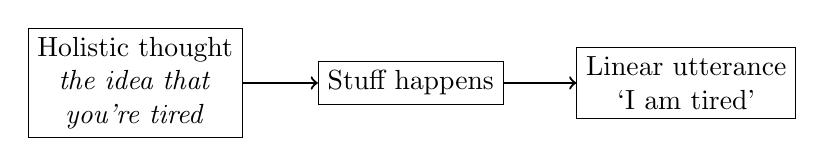
\begin{tikzpicture}[node distance=3.5cm]
            \node (holistic) [process]                    {Holistic thought \\
                                                          \emph{the idea that} \\
                                                          \emph{you're tired}};
            \node (stuff)    [process, right of=holistic] {Stuff happens};
            \node (linear)   [process, right of=stuff]    {Linear utterance \\
                                                          \uttr{I am tired}};
            \draw [arrow] (holistic) -- (stuff);
            \draw [arrow] (stuff)    -- (linear);
          \end{tikzpicture}
        \end{block}
        \begin{block}{}
          Both sentence structures and phonetic forms are arranged linearly
        \end{block}
      \end{frame}

    \subsection{\subonetwo}
      \begin{frame}{\subonetwo}
        \begin{block}{Two models}
          \begin{itemize}
            \item The utterance generator model %\parencite{fromkin_non-anomalous_1971}
            \item %\citeauthor{levelt_speaking:_1989}'s (\citeyear{levelt_speaking:_1989}) model
          \end{itemize}
        \end{block}
      \end{frame}

      \begin{frame}[t]{\subonetwo}
        \begin{block}{The utterance generator}
          Identify meaning $\rightarrow$ Select syntactic structure $\rightarrow$ Generate intonation contour $\rightarrow$ Insert content words $\rightarrow$ Insert function words \& affixes $\rightarrow$ Specify phonetic segments
        \end{block}
        \only<1>{
          \begin{block}{This is a serial model}
            \begin{itemize}
              \item \alert{Serial model}: % Serial model
A type of model for speech production or processing where steps are executed one after the other

              \item \alert{Parallel mode}: % Parallel model
A type of model for speech production or processing where steps can feed back into previous steps

            \end{itemize}
          \end{block}
        }
        \only<2>{
          \begin{block}{Example: \uttr{Peter walked down the stairs.}}
            \begin{tabular}{r @{) } l @{: } l}
              1 & Meaning     & \emph{Peter walking down the stairs in the past} \\
              2 & Structure   & [NP \_] [V \_] [P \_] [NP \_] \\
              3 & Intonation  & [NP \_] ↗[V \_] [P \_] ↘[NP \_] \\
              4 & Content     & [NP Peter] ↗[V walk] [P \_] ↘[NP stair] \\
              5 & Function    & \begin{tabular}[t]{@{} l @{}}
                                  [NP Peter] ↗[V walk-ed] [P down] \\
                                  ↘[NP the stair-s]
                                \end{tabular} \\
              6 & Phonetics   & [ˈpi.tɹ̩ ˈwɔkt ˈdaʊn ðə ˈstɛɹz]
            \end{tabular}
          \end{block}
        }
      \end{frame}

      \begin{frame}{\subonetwo}
        \begin{block}{Levelt's parallel model}
          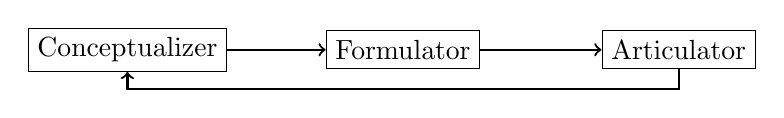
\begin{tikzpicture}[node distance=3.5cm]
            \node (concept)    [process]                   {Conceptualizer};
            \node (form)       [process, right of=concept] {Formulator};
            \node (articulate) [process, right of=form]    {Articulator};
            \draw [arrow] (concept)    -- (form);
            \draw [arrow] (form)       -- (articulate);
            \draw [arrow] (articulate) --++ (0cm, -0.5cm) -| (concept);
          \end{tikzpicture}
        \end{block}
        \begin{block}{Formulator functions}
          Grammatical encoding
          \begin{itemize}
            \item i.e., syntactic structure \& lexical expressions
          \end{itemize}
          Phonological encoding
        \end{block}
      \end{frame}

      \begin{frame}{References}
        % \printbibliography
      \end{frame}
\end{document}
